
%(BEGIN_QUESTION)
% Copyright 2007, Tony R. Kuphaldt, released under the Creative Commons Attribution License (v 1.0)
% This means you may do almost anything with this work of mine, so long as you give me proper credit

Suppose two temperature-measuring instruments are measuring the exact same process temperature, providing redundant indications inside a control room:

$$\includegraphics[width=15.5cm]{i02969x01.eps}$$

Both instruments are rather primitive: the thermocouple indicator is nothing more than an analog milli-voltmeter movement, and the filled-bulb system is a Class V arrangement with a simple bourdon tube pressure gauge mechanism used as the temperature indicator.

Now, suppose that the operator accidently bumps the thermostat in the control room, causing the control room's ambient temperature to increase by 20$^{o}$ F.  Assuming the process vessel temperature remains the same, describe the effect of elevated control room temperature on both temperature indicators, being sure to explain {\it why} for both cases.

\vskip 20pt \vbox{\hrule \hbox{\strut \vrule{} {\bf Suggestions for Socratic discussion} \vrule} \hrule}

\begin{itemize}
\item{} Some Class V filled-bulb temperature instruments are {\it compensated} to eliminate calibration errors resulting from changes in ambient temperature.  Explain how such a ``compensating'' mechanism might function -- how exactly would it sense and then compensate for room temperature?
\end{itemize}

\underbar{file i02969}
%(END_QUESTION)





%(BEGIN_ANSWER)

The thermocouple-based instrument's indication will {\it decrease} by approximately 20$^{o}$ F, while the Class V filled system's indication will {\it increase} slightly.

%(END_ANSWER)





%(BEGIN_NOTES)

The thermocouple indication will decrease because the increased control room temperature results in an increased reference junction voltage which ``takes away'' from the measurement junction's voltage.

\vskip 10pt

The filled system, being primitive, is uncompensated.  This means the mercury in the bourdon tube assembly is liable to expansion with temperature just like the mercury in the bulb.  Thus, when the control room temperature increases, the mercury inside the bourdon tube expands and causes the bourdon tube to elongate, showing increased temperature.

%INDEX% Measurement, temperature: filled-bulb system
%INDEX% Measurement, temperature: thermocouple

%(END_NOTES)


